\documentclass[twoside,12pt,openright,final,english]{memoir}

\usepackage{graphicx}
\graphicspath{{./images-1600x1200/}}

\usepackage{color}
\usepackage[usenames,dvipsnames,svgnames,table]{xcolor}

%%% PAGE, STOCK, AND MARGIN SIZE %%%
% 8.5" by 11
\setstocksize{27.94cm}{21.59cm} % { height }{ width }
\settrimmedsize{\stockheight}{\stockwidth}{*}

%\settypeblocksize{ height }{ width }{ ratio }
\settypeblocksize{23.5cm}{*}{*}

%\setlrmarginsandblock{ spine }{ edge }{ ratio }
% make the spine have more space than outer edge
\setlrmarginsandblock{*}{2.0cm}{1.0}

% The command \setulmargins can be used to specify the upper and lower mar-
% gins where the heights of the page and the typeblock are fixed.
% \setulmargins{ upper }{ lower }{ ratio }
\setulmargins{1.5cm}{*}{*}

%\isopage
%\checkandfixthelayout
\checkandfixthelayout[fixed]
%%% END PAGE, STOCK, AND MARGIN SIZE %%%

\usepackage[english]{babel}
% WTF?
\usepackage{ucs}

%%% PDFLATEX %%%
% fixes "no room for a new \count" error
\usepackage{etex}
\usepackage[protrusion,expansion,spacing,kerning,babel,final]{microtype}
\usepackage[utf8x]{inputenc}
%%% END FONT FONT FONT %%%

%%% LEDMAC %%%
\usepackage{ledmac}
%%% END LEDMAC %%%

%%% PAGE STYLE %%%
\makepagestyle{jebstyle}
\pagestyle{jebstyle}

%%% jebinski CHAPTER STYLE %%%
\makechapterstyle{jebinski}{%
% Clear out the chapter name (e.g. capítulo)
  \renewcommand*{\printchaptername}{}
% Clear out the chapter number
  \renewcommand*{\printchapternum}{}
% Set chapter font
  \renewcommand*{\chaptitlefont}{\normalfont\large\scshape}
  \renewcommand*{\printchaptertitle}[1]{%
     \hrule\vskip\onelineskip \centering \chaptitlefont{##1}\par}
  \renewcommand*{\afterchaptertitle}{\vskip\onelineskip \hrule\vskip
     \afterchapskip}
}
%%% END jebinski CHAPTER STYLE %%%

%%% FORMATTING KLUDGES %%%
% fewer overfull lines compared with \fussy and fewer obvious
% large interword spaces than with \sloppy.
\midsloppy
% "fix" for Overfull \hbox
%\emergencystretch=8pt
\setlength{\emergencystretch}{3em}  % 3em
% Prints out a block on overfull hbox lines
%\overfullrule=5pt
%
% \tolerance is a paragraph parameter, probably ignored here
\tolerance=5000 % allow looser spacing 
%\tolerance=95000 % allow waaay looser spacing 
%
% 10000 almost prevents hyphenation. What's default?
\hyphenpenalty=500 % 500 seems reasonable
%
%the default \flushbottom
%\sloppypar
\setlength{\topskip}{1.6\topskip}
\checkandfixthelayout
%\sloppybottom
\raggedbottom

%%%%%%%% WIDOWS AND ORPHANS %%%%%%%%%%%
\widowpenalty=10000
\clubpenalty=10000
%%%%%%%% END WIDOWS AND ORPHANS %%%%%%%%%%%
%%% END FORMATTING KLUDGES %%%

%%% Fancy dings %%%
\usepackage{pifont}
%%% END OF PREAMBLE %%%

\begin{document}

%%% CHAPTER STYLE %%%
\chapterstyle{jebinski} % defined in preamble
%%% END CHAPTER STYLE %%%

%%% BEGIN MAINMATTER %%%
\mainmatter*
% turn off page numbering
\pagenumbering*{gobble}
\setcounter{figure}{0}
\renewcommand{\thefigure}{\arabic{figure}}

%%% UNPACKING %%%
\def\topblockvspace{0.0}
\centering
{\huge \scshape Unpacking Instructions}\\[\baselineskip]

\begin{enumerate}

\begin{figure}[h]
\centering
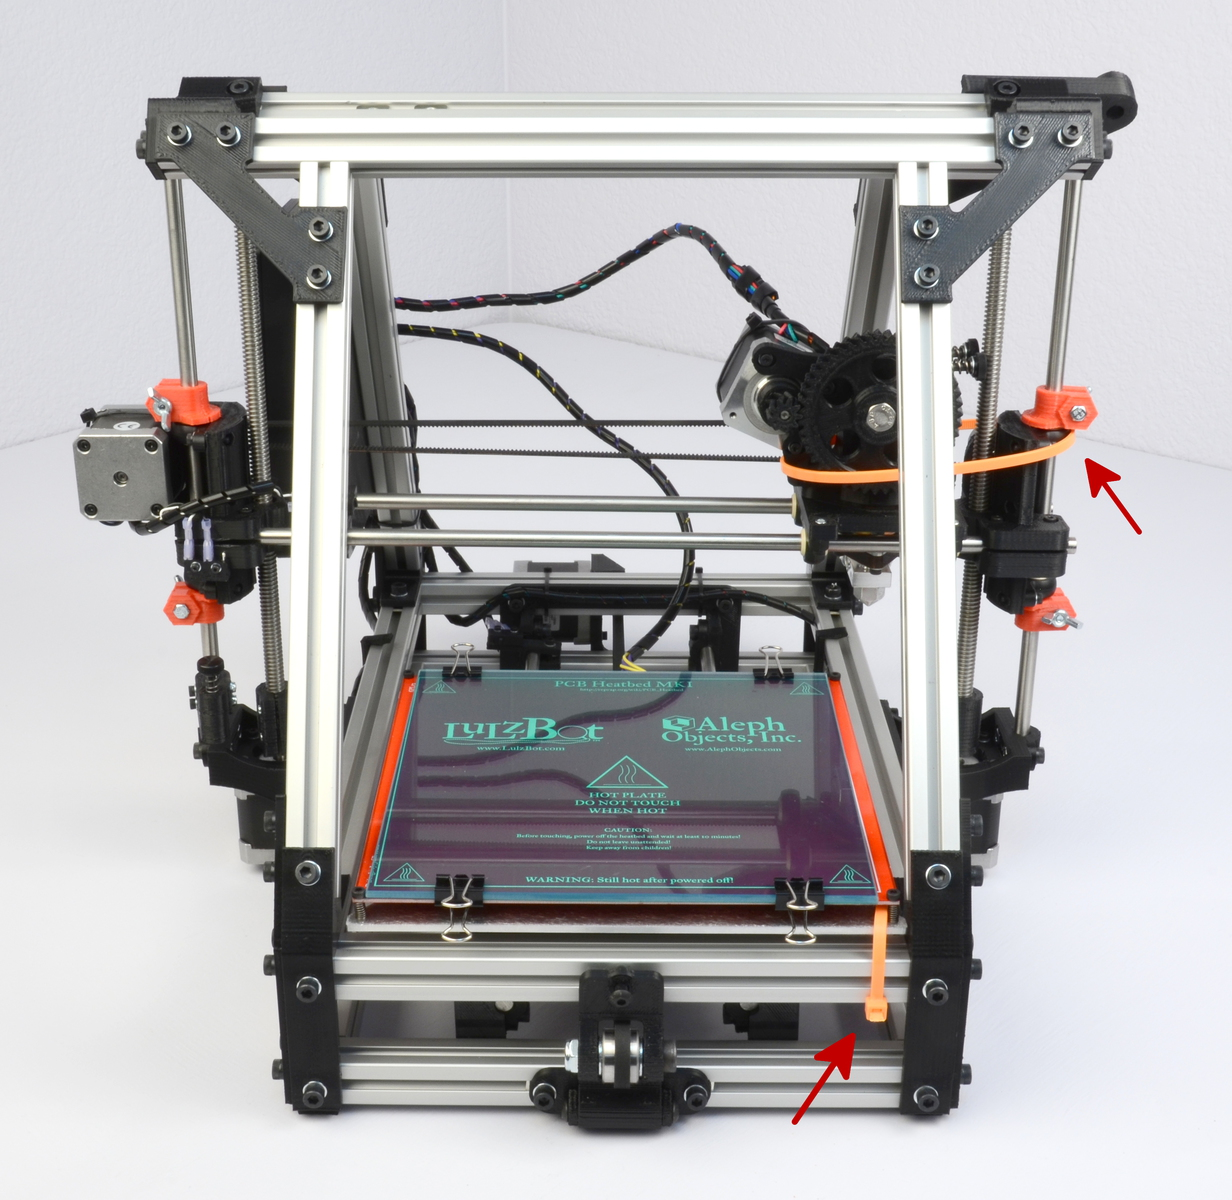
\includegraphics[keepaspectratio=true,angle=0,height=0.3\textheight,width=1.0\textwidth]{zip_ties.jpg}
\caption{Orange Zip Ties}
\label{fig:zip_ties}
\end{figure}

\item Remove the plastic bag containing instructions, cords, and small parts.

\item Remove the top foam padding. 

\item Slowly remove the two smaller foam pads. One of these pads will contain the plastic filament spool and plastic filament guide. The other pad will contain the 5lb coil of ABS plastic filament. Remove these items from the box with the two small foam pads.

\item Remove the white power supply box and the black tool bag. These items are along opposite sides of the printer.

\item Grab the top of the wrapped printer on the top center where you will feel two lengths of square aluminum tubing. Holding the top two tubes, SLOWLY pull the printer upwards out of the box. The two large side foam pads should fall off when the printer is out of the box.

\item Set you printer on a stable level surface.

\item Gently unwrap the pink ESD plastic covering the printer. Remove the rolled sheet of PET tape from below the print bed. Gently lift the printer to slide the plastic wrapping from under the printer. 

\begin{figure}[h]
\centering
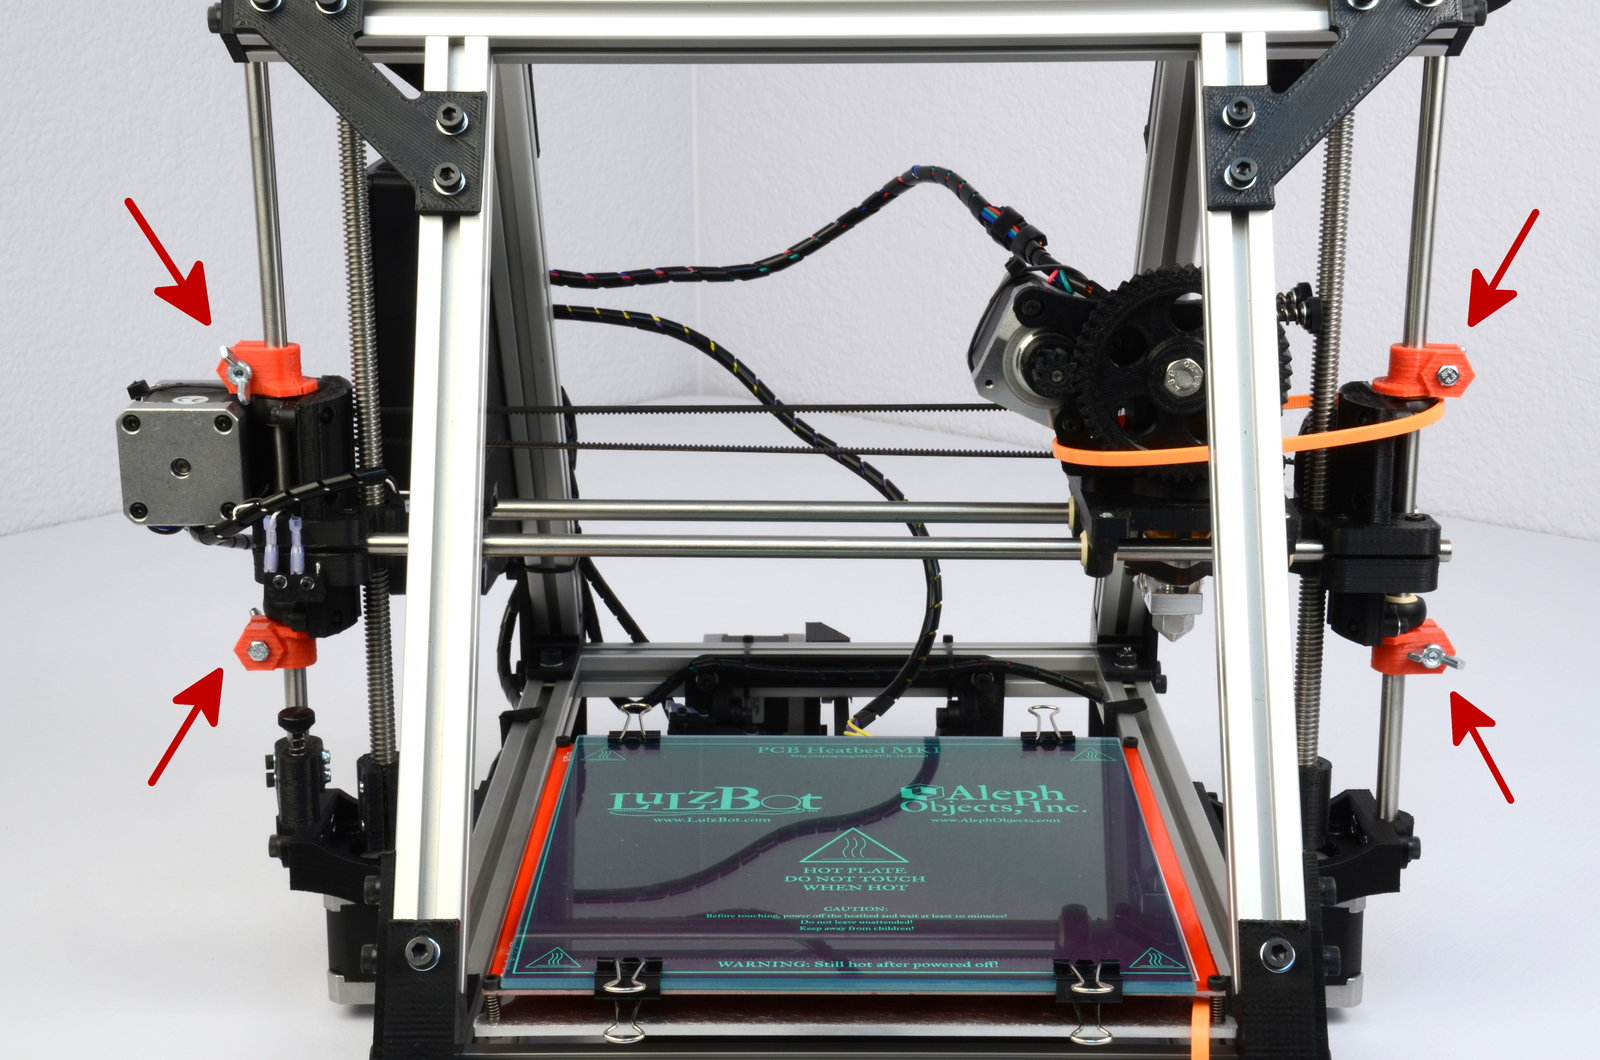
\includegraphics[keepaspectratio=true,angle=0,height=0.3\textheight,width=1.0\textwidth]{shipping_clamps.jpg}
\caption{Red Shipping Clamps}
\label{fig:shipping_clamps}
\end{figure}

\item Using scissors or wire cutters, cut and remove the two ORANGE plastic zip ties
(Fig. \ref{fig:zip_ties})
. One zip tie is located on the bottom front of the printer on the print bed. The other zip tie is around the extruder carriage and X axis. Make sure to not cut any of the surrounding wires or belts.

\item Find the item list attached to the plastic bag of parts. Before you move on to setting up your printer make sure all of the items on the list are in your package.

\begin{figure}[h]
\centering
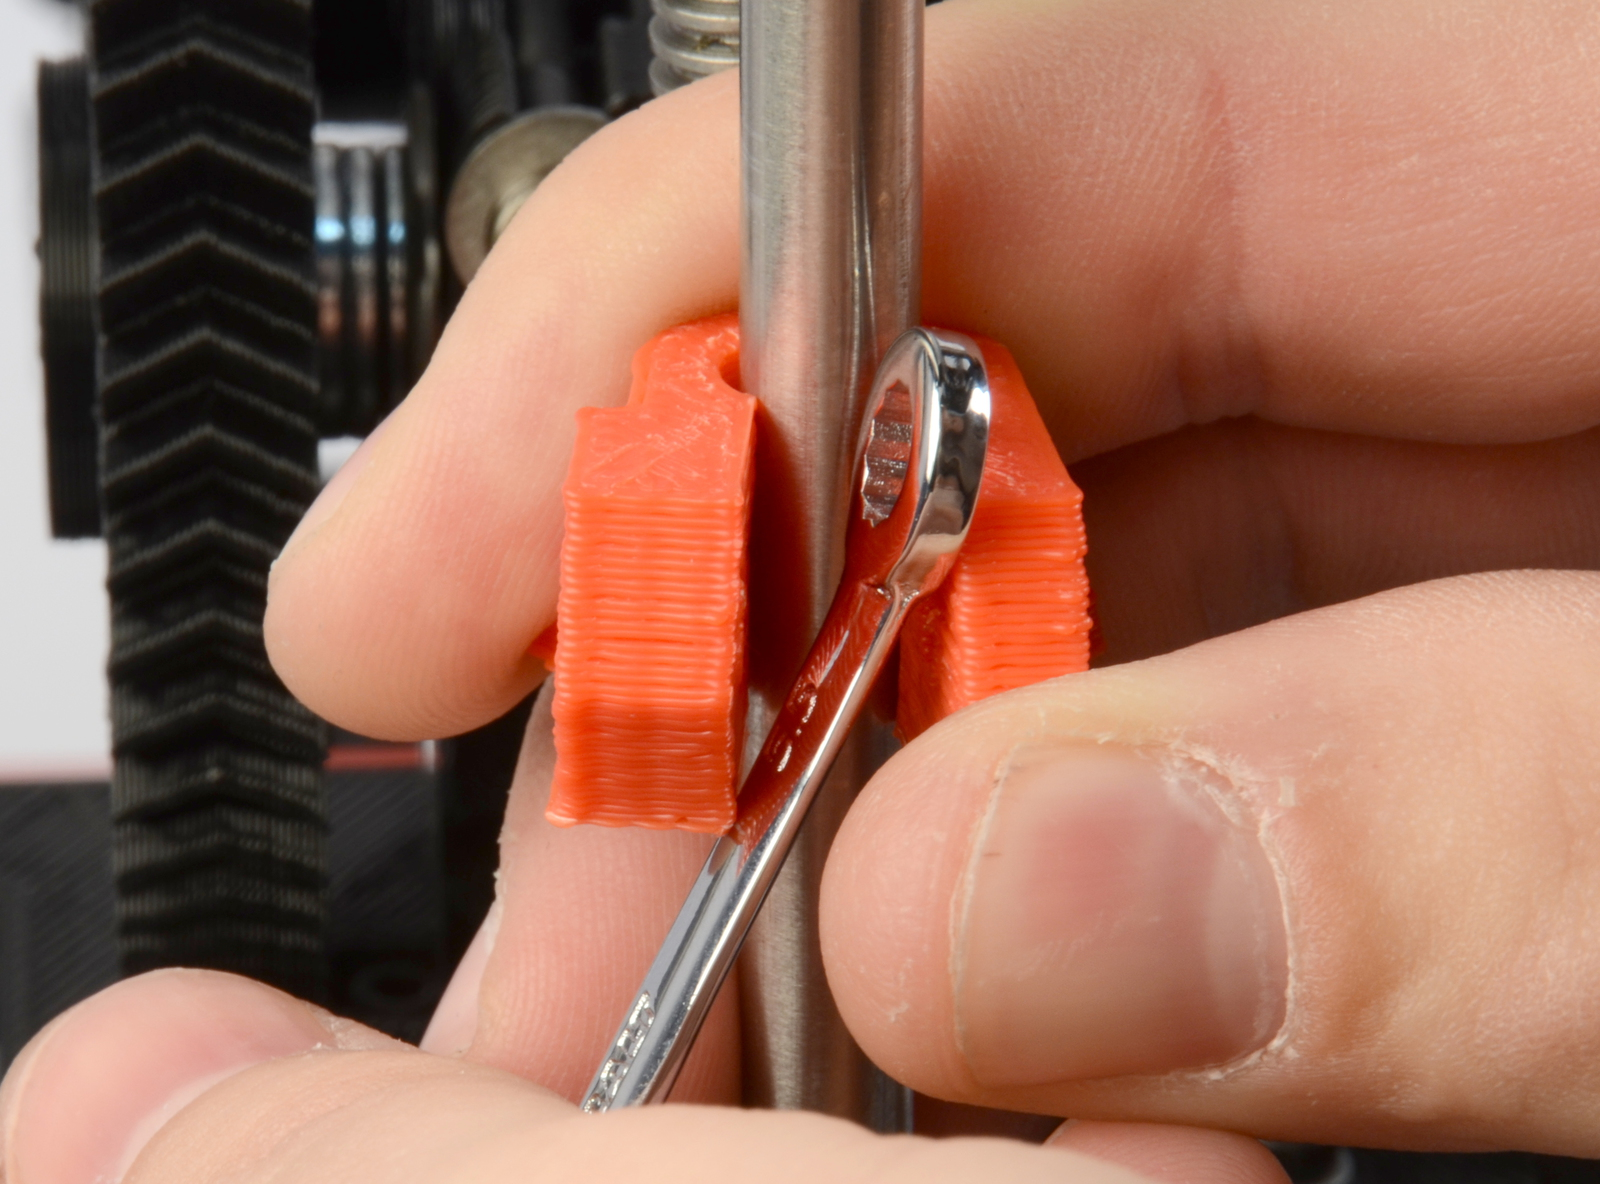
\includegraphics[keepaspectratio=true,angle=0,height=0.3\textheight,width=1.0\textwidth]{shipping_clamps_pry.jpg}
\caption{Using a wrench to pry off the shipping clamps}
\label{fig:shipping_clamps_pry}
\end{figure}

\item Remove the four red shipping clamps above and below the x-end motor mount and idler
(Fig. \ref{fig:shipping_clamps}).

\item Loosen and remove the wing nut and screw on each of the four clamps. Remove each of the four clamps by popping them off of the smooth rod. Use a screwdriver or wrench to pry open and remove the clamps if you have trouble removing them by hand (Fig. \ref{fig:shipping_clamps_pry}). Keep the clamps and hardware for future use if you need to ship or transport your printer.

\item Remove the blue tape from two sides of the print surface. Make sure to not remove the green PET tape on the glass print surface. The PET tape helps keep the print attached to the print surface during printing.

\end{enumerate}
%%% END UNPACKING %%%

%%% END MAINMATTER %%%

\end{document}

